\noindent
De acuerdo con lo expuesto en la Sección \ref{sec:plataformas},
empleamos CARLA como entorno de simulación para nuestros experimentos.
El escenario de estacionamiento incluye un vehículo con el objetivo de estacionarse y un área con cajones marcados.
La posición inicial del vehículo se varía de forma controlada entre ejecuciones.
La cámara frontal se monta en la zona del retrovisor a altura conocida,
y se recopilan secuencias de imágenes para alimentar el pipeline de detección de líneas,
estimación de puntos de fuga y ajuste de retícula por RANSAC.
La Figura~\ref{fig:simulation-design} muestra un ejemplo del diseño del entorno.

\begin{figure}[!ht]
    \centering
    \begin{subfigure}{0.4\textwidth}
        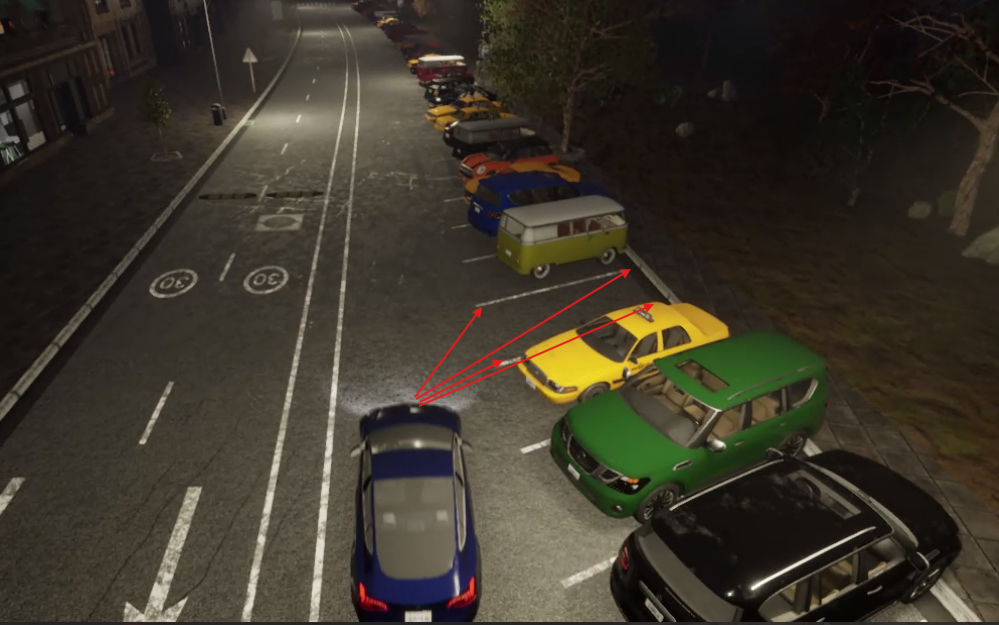
\includegraphics[width=\textwidth]{img/distances}\label {fig:distances}
    \end{subfigure}
    \begin{subfigure}{0.4\textwidth}
        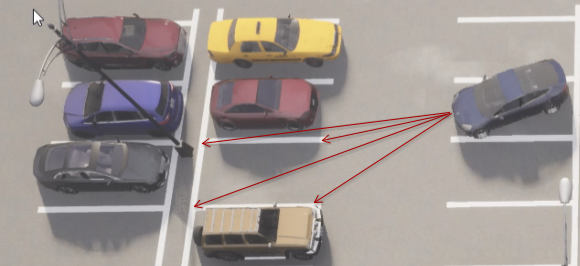
\includegraphics[width=\textwidth]{img/distances2}\label {fig:distances2}
    \end{subfigure}

    \caption{Diseño del entorno de simulación en CARLA.}
    \label{fig:simulation-design}
\end{figure}

\noindent
La Figura~\ref{fig:camera-view} ilustra ejemplos de la vista de la cámara frontal desde la ubicación definida.

\begin{figure}[!ht]
    \centering
    \begin{subfigure}{0.4\textwidth}
        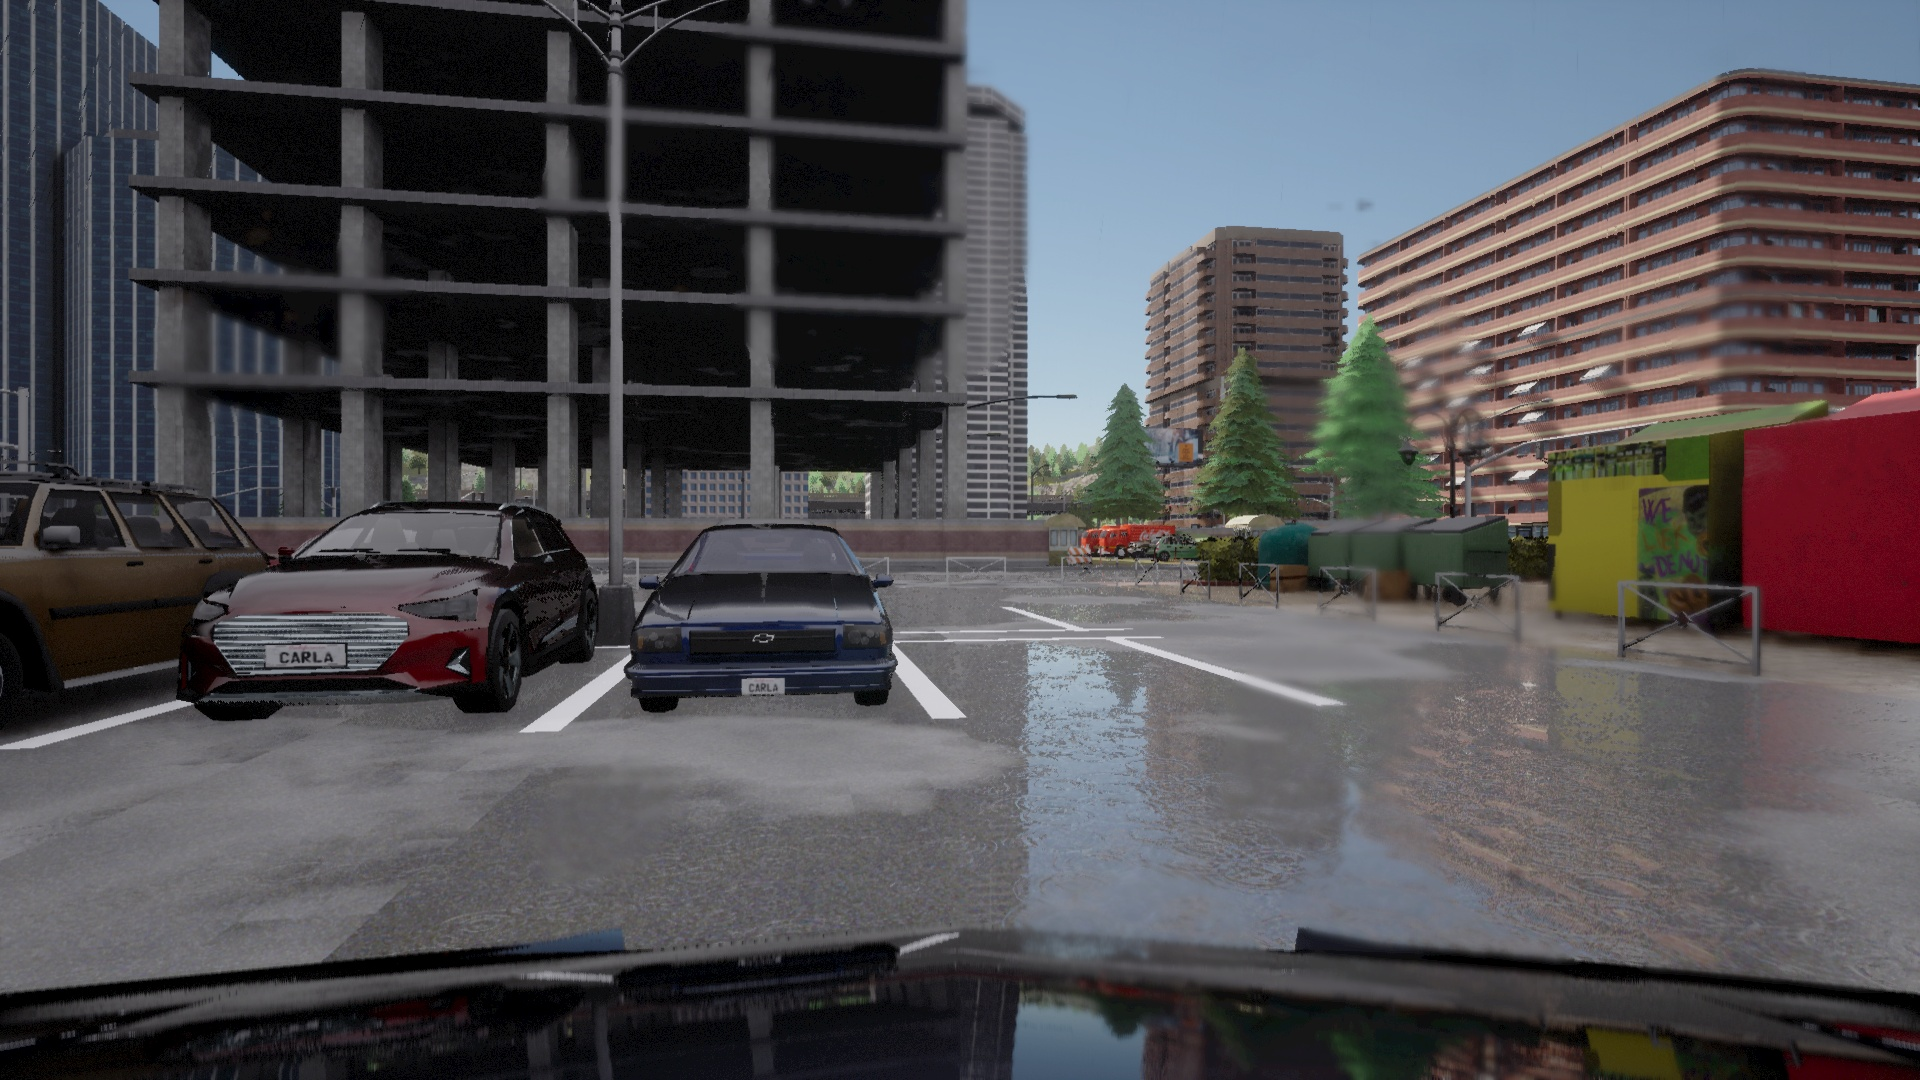
\includegraphics[width=\textwidth]{img/mirrow_camara_ex}\label {fig:camara}
    \end{subfigure}
    \begin{subfigure}{0.4\textwidth}
        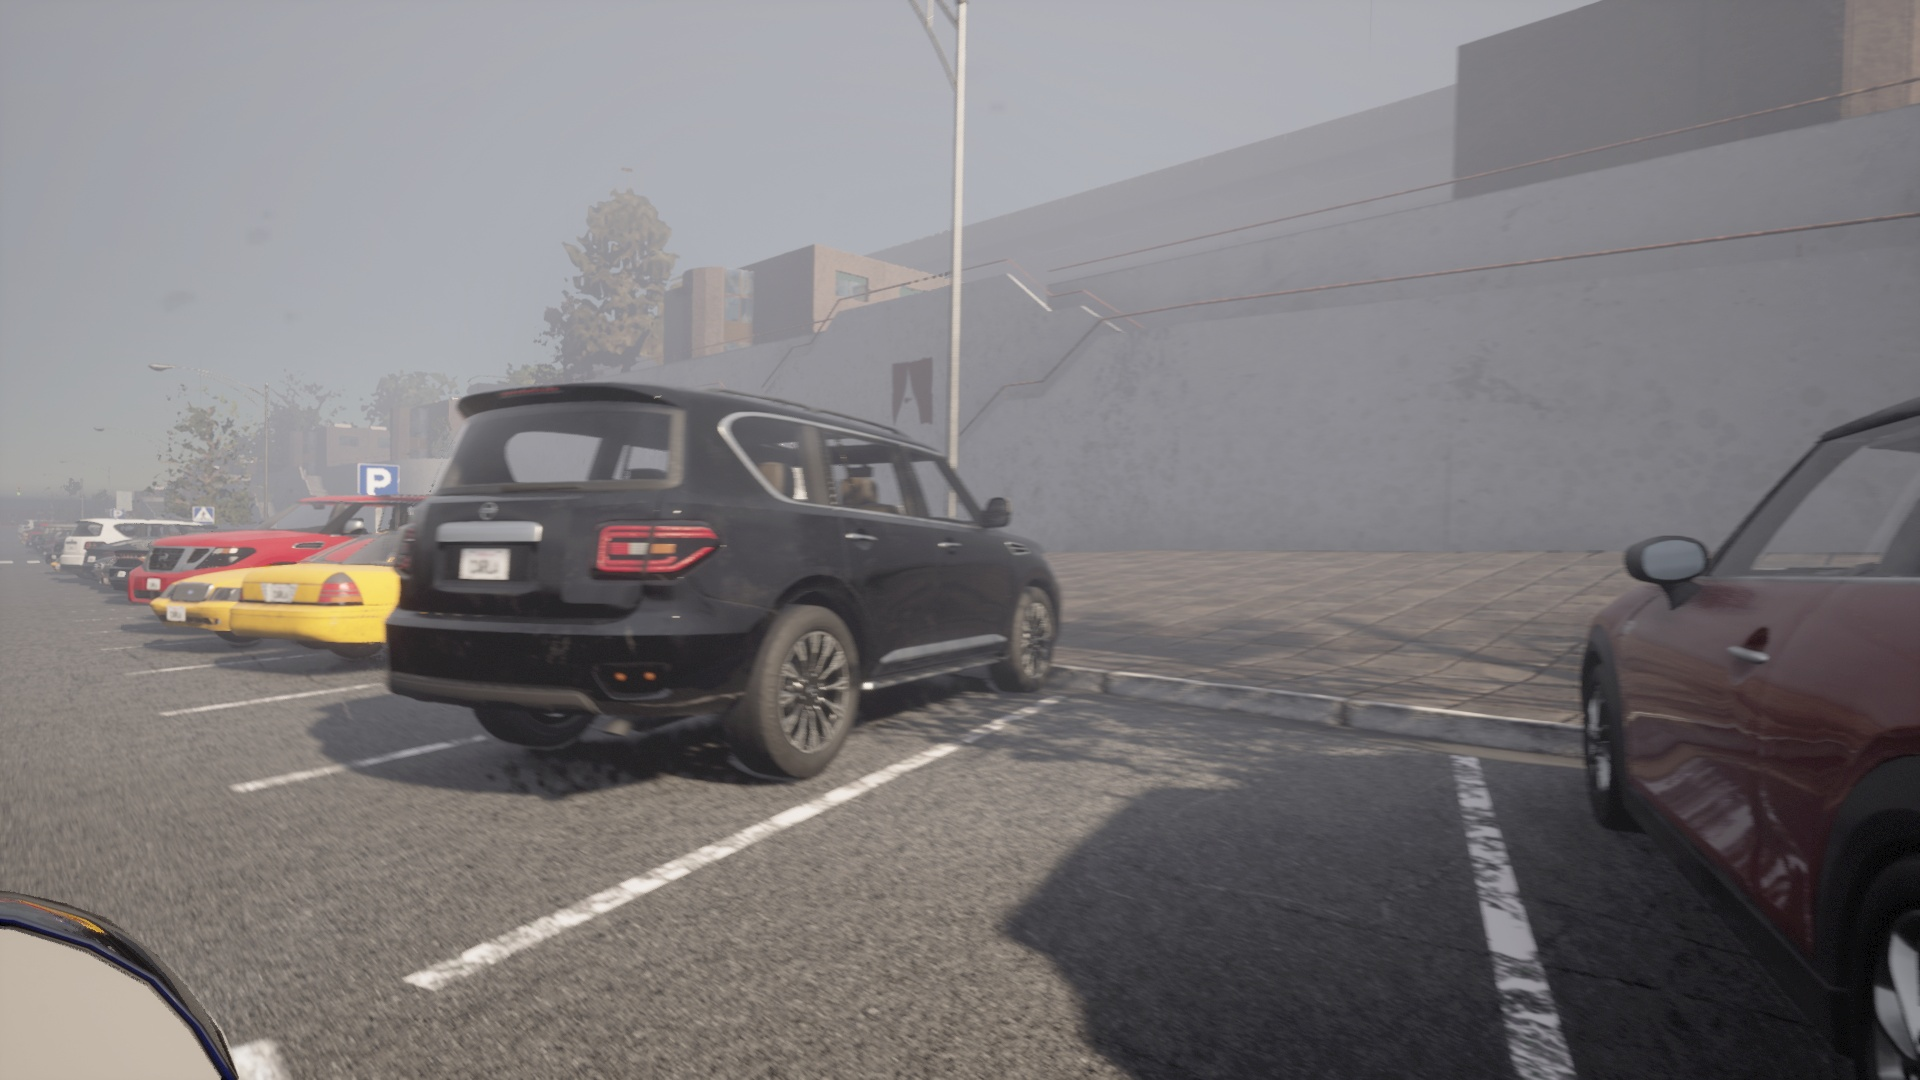
\includegraphics[width=\textwidth]{img/mirrow_camara_ex2}\label {fig:camara2}
    \end{subfigure}
    \caption{Vista de la cámara en el entorno de simulación.}
    \label{fig:camera-view}
\end{figure}




